%% FEUP THESIS STYLE for LaTeX2e
%% how to use feupteses (portuguese version)
%%
%% FEUP, JCL & JCF, 31 Jul 2012
%%
%% PLEASE send improvements to jlopes at fe.up.pt and to jcf at fe.up.pt
%%

%%========================================
%% Commands: pdflatex tese
%%           bibtex tese
%%           makeindex tese (only if creating an index) 
%%           pdflatex tese
%% Alternative:
%%          latexmk -pdf tese.tex
%%========================================

\documentclass[11pt,a4paper,twoside,openright]{report}

%% For iso-8859-1 (latin1), comment next line and uncomment the second line
\usepackage[utf8]{inputenc}
%\usepackage[latin1]{inputenc}

%% Portuguese version

%% MIEIC options
\usepackage[portugues,mieic]{feupteses}
%\usepackage[portugues,mieic,juri]{feupteses}
%\usepackage[portugues,mieic,final]{feupteses}
%\usepackage[portugues,mieic,final,onpaper]{feupteses}

%% Options: 
%% - portugues: titles, etc in portuguese
%% - onpaper: links are not shown (for paper versions)
%% - backrefs: include back references from bibliography to citation place

%% Uncomment the next lines if side by side graphics used
%\usepackage[lofdepth,lotdepth]{subfig}
%\usepackage{graphicx}
%\usepackage{float}

%% Include color package
\usepackage{color}
\definecolor{cloudwhite}{cmyk}{0,0,0,0.025}

%% Include source-code listings package
\usepackage{listings}
\lstset{ %
 language=C,                        % choose the language of the code
 basicstyle=\footnotesize\ttfamily,
 keywordstyle=\bfseries,
 numbers=left,                      % where to put the line-numbers
 numberstyle=\scriptsize\texttt,    % the size of the fonts that are used for the line-numbers
 stepnumber=1,                      % the step between two line-numbers. If it's 1 each line will be numbered
 numbersep=8pt,                     % how far the line-numbers are from the code
 frame=tb,
 float=htb,
 aboveskip=8mm,
 belowskip=4mm,
 backgroundcolor=\color{cloudwhite},
 showspaces=false,                  % show spaces adding particular underscores
 showstringspaces=false,            % underline spaces within strings
 showtabs=false,                    % show tabs within strings adding particular underscores
 tabsize=2,	                    % sets default tabsize to 2 spaces
 captionpos=b,                      % sets the caption-position to bottom
 breaklines=true,                   % sets automatic line breaking
 breakatwhitespace=false,           % sets if automatic breaks should only happen at whitespace
 escapeinside={\%*}{*)},            % if you want to add a comment within your code
 morekeywords={*,var,template,new}  % if you want to add more keywords to the set
}

%% Uncomment next line to set the depth of sectional units listed in the toc
%\setcounter{tocdepth}{3}

%% Uncomment to create an index (at the end of the document)
%\makeindex

%% Path to the figures directory
%% TIP: use folder ``figures'' to keep all your figures
\graphicspath{{figures/}}

%%----------------------------------------
%% TIP: if you want to define more macros, use an external file to keep them
%some macro definitions

% format
\newcommand{\class}[1]{{\normalfont\slshape #1\/}}

% entities
\newcommand{\Feup}{Faculdade de Engenharia da Universidade do Porto}

\newcommand{\svg}{\class{SVG}}
\newcommand{\scada}{\class{SCADA}}
\newcommand{\scadadms}{\class{SCADA/DMS}}

%%----------------------------------------

%%========================================
%% Start of document
%%========================================
\begin{document}

%%----------------------------------------
%% Information about the work
%%----------------------------------------
\title{Título da Dissertação}
\author{Maria João Barreira}

%% Uncomment next line for date of submission
%\thesisdate{31 de Julho de 2008}

%% Uncomment next line for copyright text if used
%\copyrightnotice{Nome do Autor, 2008}

\supervisor{Orientador}{Teresa Galvão}

%% Uncomment next line if necessary
%\supervisor{Co-orientador}{Nome de Outro Orientador}

%% Uncomment committee stuff in the final version
%\committeetext{Aprovado em provas públicas pelo Júri:}
%\committeemember{Presidente}{Nome do presidente do júri}
%\committeemember{Arguente}{Nome do arguente do júri}
%\committeemember{Vogal}{Nome do vogal do júri}
%\signature

%% Specify cover logo (in folder ``figures'')
\logo{uporto-feup.pdf}

%% Uncomment next line for additional text below the author's name (front page)
%\additionalfronttext{Preparação da Dissertação}

%%----------------------------------------
%% Preliminary materials
%%----------------------------------------

% remove unnecessary \include{} commands
\begin{Prolog}
  %!TEX root = mieic.tex
\chapter*{Resumo}

Os ecrãs públicos digitais têm cada vez mais uma forte presença no nosso dia-a-dia, contudo poucos são os que permitem uma manipulação direta por parte do utilizador. Atualmente, a sua função é maioritariamente publicitar determinado serviço ou produto, e a maior parte das vezes até passam despercebidos aos transeuntes.

É importante reconhecer o valor de quem interage com o ecrã e permitir um desenvolvimento mais fácil de aplicações ricas, que propiciem uma interação eficaz por parte de um ou mais utilizadores. 

Aliando o crescente uso de dispositivos móveis, como \textit{smartphones} e \textit{tablets}, aos recentes avanços tecnológicos existentes nos ecrãs públicos digitais, este projeto apresentava como principais objetivos a criação de uma \textit{framework} que facilite o desenvolvimento de aplicações de cariz público e a implementação de alguns exemplos destas aplicações, que permitam a utilização da \textit{framework} desenvolvida.

A \textit{framework} desenvolvida encontra-se orientada a objetos, sendo composta por 4 classes distintas. As subclasses representam os tipos de controlos que o programador terá disponíveis e poderá implementar na sua aplicação. Neste caso, foram desenvolvidos 3 diferentes tipos de widgets, que permitirão ao utilizador final interagir com a aplicação.

Como exemplo de aplicação foi implementado o clássico jogo da \textit{Snake}. Uma vez que não havia necessidade de desenvolver o jogo de raíz, foi necessário pesquisar por um exemplo em \textit{html} e \textit{javascript} ao qual se pudessem adaptar os controlos da \textit{framework}. Apesar de existirem um grande número de opções, foi escolhido o jogo referido, uma vez que é um jogo bastante conhecido, que não necessita de grandes explicações e num modo multi-jogador torna-se competitivo.

Não só no final, mas também ao longo do desenvolvimento, ocorreu a realização de alguns testes. Os testes realizados ao longo do desenvolvimento permitiram saber se a funcionalidade implementada fazia realmente o que é desejado, obtendo de forma rápida \textit{feedback} do trabalho acabado de realizar, prevenindo erros futuros semelhantes e trabalho desnecessário. 

No final foi pedido a 3 estudantes do MIEIC que integrassem a \textit{framework} desenvolvida com soluções \textit{open source} recorrendo à mesma para a definição dos respetivos controlos.


\chapter*{Abstract}

The presence of digital public displays in urban landscapes has increased, however only few of them allow a direct-manipulation to passersby. Nowadays, the main feature is to advertise a service or a product and often people ignore them. 

It is important to be centered in the final user and allow to developers an easier development of applications providing an efficient interaction for one or more users. 

Combining the growing use of mobile devices, such as smartphones and tablets, with the latest technological advances in existing public digital displays, this project had as main goals the creation of a framework that eases the development of public applications and the implementation of some examples allowing the use of the developed framework.

The developed object-oriented framework heavily relies in inheritance consisting of four distinct classes, one of them being an interface, that is the abstract representation of a control. The subclasses represent the types of controls that the developer will have available and can implement in an application. In this case, three different types of widgets, that allow the final user to interact with the application, have been developed.

As an example of application, it was implemented the classic game of Snake. Since there was no need to create the game, it was necessary to search for an example in HTML and JavaScript which it could apply the controls of framework. Although there were a large number of options, this game was chosen because it is well-known and, henceforth it does not need much explanation. Besides, in multiplayer mode the game becomes competitive.

Not only at the end, but also throughout development, some tests occurred. Tests during the development allowed whether the implemented functionality was the desired or not, quickly getting feedback from the most recent changes on the work, preventing similar future errors and unnecessary work.

At the end, three students from MIEIC were asked to incorporate the framework on open-source solutions using it for the respective controls implementation. % the abstract
  \chapter*{Agradecimentos}
%\addcontentsline{toc}{chapter}{Agradecimentos}



\vspace{10mm}
\flushleft{Maria João Barreira}
  % the acknowledgments
  %!TEX root = mieic.tex

\cleardoublepage
\thispagestyle{plain}

\vspace*{8cm}

\begin{flushright}
   \textsl{``You should be glad that bridge fell down. \\
           I was planning to build thirteen more to that same design''} \\
\vspace*{1.5cm}
           Isambard Kingdom Brunel
\end{flushright}
    % initial quotation if desired
  \cleardoublepage
  \pdfbookmark[0]{Conteúdo}{contents}
  \tableofcontents
  \cleardoublepage
  \pdfbookmark[0]{Lista de Figuras}{figures}
  \listoffigures
  \cleardoublepage
  \pdfbookmark[0]{Lista de Tabelas}{tables}
  \listoftables
  %!TEX root = mieic.tex
\chapter*{Abreviaturas e Símbolos}
%\addcontentsline{toc}{chapter}{Abbreviations}
\chaptermark{ABREVIATURAS E SÍMBOLOS}

\begin{flushleft}
\begin{tabular}{l p{0.8\linewidth}}
IHP     & Interação Humano-Computador\\
DCU     & Desenvolvimento Centrado no Utilizador\\
API		& \textit{Application programming interface}
\end{tabular}
\end{flushleft}

  % the list of abbreviations used
\end{Prolog}

%%----------------------------------------
%% Body
%%----------------------------------------

\StartBody

%% TIP: use a separate file for each chapter
%!TEX root = mieic.tex
\chapter{Introdução} \label{chap:intro}

\section*{}
 
Esta dissertação, tem como tema \textit{Remote, direct-manipulation interaction for multi-user, web-based public display applications} e foi proposta pelo CITAR\footnote{Centro de Investigação em Ciência e Tecnologia das Artes, http://artes.ucp.pt/citar/} da Universidade Católica.  

\section{Contexto/Enquadramento} \label{sec:context}

Na atualidade, é cada vez maior o número de ecrãs públicos existentes em diversos cenários urbanos, sejam eles paragens de transportes públicos, salas de espera ou outras zonas mais movimentadas. No entanto, a maioria destes apenas é utilizada como meio de divulgação de determinado produto ou serviço, não permitindo ao transeunte interagir com o mesmo. A população já está habituada à sua presença, classificando-os muitas vezes como objetos inúteis, podendo facilmente passar despercebidos. 

Este cenário pode ser alterado, pois os recentes avanços da tecnologia podem proporcionar aos utilizadores interação com estes ecrãs através da manipulação direta dos mesmos, usando para isso o seu dispositivo móvel.

Apesar de já existir algum desenvolvimento nesta área, alterar o estado atual dos ecrãs em algo completamente novo requer algum investimento tecnológico e inovação.

Uma pesquisa mais cuidada revela que já começa a ser comum, em áreas mais movimentadas, como estações de comboios ou praças públicas a possibilidade de as pessoas interagirem com diversos ecrãs. Existem diferentes maneiras pelas quais esta interação é possível, como por exemplo através do toque, leitura de \textit{QR code}, introdução de um código, ou usando um \textit{kinnect} inserido no próprio ecrã. 

Nigel Davies~\cite{Davies2012b}, em \textit{Open Display Networks: A Communications Medium for the 21st Century}, compara a situação dos ecrãs públicos com os \textit{smartphones}, afirmando que a inovação ocorre quando são criados sistemas livres que encorajam a inovação e incentivam a um maior desenvolvimento de novos produtos.

\section{Projeto e Objetivos} \label{sec:proj}

O tema proposto tem como objetivo principal desenvolver e validar uma arquitetura que permita uma interação baseada no paradigma da manipulação directa, por outras palavras, tal como o nome indica representa uma interação que ocorre de forma direta, em que o utilizador se apercebe das alterações no exato momento.  

No final pretende-se obter uma \textit{framework} que facilite a criação de aplicações para ecrãs públicos, baseadas no paradigma acima descrito, bem como algumas aplicações exemplos que sejam construídas com base na API desenvolvida.

\section{Desafios} \label{sec:goals}

Como já foi referido anteriormente cada vez mais, em locais públicos existem diversos ecrãs, contudo a sua maioria apenas serve para publicitar determinado produto ou serviço. 

Esta é uma área nova, em constante desenvolvimento, em que há a possibilidade de estabelecer alguns conceitos de referência para o futuro.

Os ecrãs públicos estão situados em zonas estratégicas, encontrando-se maioritariamente localizados em zonas onde existe uma maior concentração de pessoas, sendo também importante estudar a possibilidade de uma interação por parte de mais do que  em vez de individual.

O presente projeto apresenta um lado desafiante que leva à procura de soluções para o desenvolvimento de aplicações web, que suportem uma interação por múltiplos utilizadores, usando para isso o seu próprio dispositivo móvel, levando também a pensar nos tipos de controlo que deverão estar disponíveis. 

Existem, para além dos desafios acima mencionados, outros aos quais poderá ser possível dar uma resposta, será, por exemplo, importante perceber de que modo a infra-estrutura da rede pode influenciar o correto funcionamento das aplicações, bem como se no mesmo ecrã poderá existir mais do que uma aplicação ou ainda se para cada aplicação existe a necessidade de haver um servidor diferente. 

Este trabalho irá também permitir o desenvolvimento de aplicações interativas mais ricas, abrindo o leque de possibilidades de configuração e interação com este tipo de aplicações. 

\section{Estrutura da Dissertação} \label{sec:struct}

Este relatório apresenta para além da introdução mais seis capítulos.

No capítulo~\ref{chap:biblio}, é descrito o estado da arte e são
apresentados trabalhos relacionados. 

No capítulo~\ref{chap:metod}, é apresentada a metodologia a usar no desenvolvimento do projeto, seguido do capítulo~\ref{chap:sol}, onde se descreve pormenorizadamente a solução implementada e as  tecnologias usadas para alcançar os objetivos propostos.

No capítulo~\ref{chap:testes} são descritos os testes realizados e as conclusões tiradas a partir dos mesmos, sendo realizada uma discussão e análise crítica do produto desenvolvido no capítulo~\ref{chap:disc}.

Por último, capítulo~\ref{chap:concl}, o relatório termina com uma análise conclusiva e possíveis melhoramentos futuros.
 
%!TEX root = mieic.tex
\chapter{Revisão Bibliográfica} \label{chap:biblio}

\section*{}

A interação com ecrãs públicos não é um tema novo, deste modo já existem diversas abordagens que podem ser usadas nas aplicações desenvolvidas para os mesmos.
	
Neste segundo capítulo são referidas soluções tecnológicas usadas nos diversos projetos que poderão ser utilizadas no corrente tema, bem como requisitos a considerar neste tipo de aplicações.

São também mencionados alguns trabalhos relacionados com o tema de forma a comparar o que existe desenvolvido na área referida com os problemas em aberto que ainda podem ser solucionados. 

\section{Ecrãs Públicos Interativos}

A interação com os grandes ecrãs pode ser diferenciada em três diferentes domínios: pessoal, semi-público e público~\cite{Ballagas}. Ecrãs pessoais permitem a um único utilizador visualizar e processar uma grande quantidade de informação ao mesmo tempo. Ecrãs semi-públicos encontram-se situados  num ambiente controlado como  por exemplo salas de reuniões onde apenas um número limitado de pessoas regularmente interage, normalmente usando apenas um ecrã com aplicações de grupo. Ecrãs públicos encontram-se tipicamente localizados em áreas “abertas”, usualmente em ambientes com grande movimento onde as pessoas passam e têm de esperar algum tempo, como estações de comboio, aeroportos ou parques.

Em ~\cite{Ballagas} são identificadas alguma considerações especificas para técnicas de interação para ecrãs públicos, referindo a vontade espontânea de o utilizador interagir com o ecrã, a facilidade de o utilizador “transportar” as ferramentas necessárias para que a interação seja possível, pois existem mecanismos que permitem ao utilizador interagir sem qualquer dispositivo adicional e outros que exigem que o utilizador possua determinado equipamento, as considerações de limpeza e saúde associadas à técnica de interação, como a condição física do ecrã. Este aspeto poderá ter um impacto quer positivo, quer negativo no uso dos respetivos ecrãs. Também é referido o número de mãos que serão necessárias para a operação, sendo um aspeto relevante uma vez que, a maior parte das vezes, o transeunte precisa das suas mãos para carregar os seus bens, a possibilidade de a técnica de interação suportar mais do que um utilizador ao mesmo tempo, o grau de segurança e privacidade esperados quando se interage com um ecrã em público e ainda a necessidade de um serviço regular de modo a manter o sistema operacional e um aparência que seja atrativa ao seu uso.

Os ecrãs públicos tendem a possuir monitores maiores, o que pode resultar em alguns benefícios, dá maior liberdade aos programadores uma vez que a capacidade gráfica é superior à do ecrã do telemóvel, torna possível um maior número de movimentos para os participantes, cria uma atmosfera mais rica socialmente permitindo alguma interação social em diferentes cenários urbanos ~\cite{Vajk2008b}.

\subsection{Requisitos para um interação pública} \label{batik} 

Tal como já foi referido anteriormente no final do desenvolvimento deste projeto é desejado que seja mais fácil para os programadores, desenvolver aplicações que permitam a interação com ecrãs públicos, isto implica a abordagem de diversos requisitos. Segundo~\cite{Cardoso2012g} alguns desses requisitos são comuns a outros sistemas interativos, mas outros são específicos de ecrãs públicos, fazendo referência a:

\textbf{Múltiplos mecanismos de interação} - uma interação em ecrãs públicos pode usar múltiplos mecanismos de entrada, como SMS, email, Bluetooth, Twitter, gestos ou movimento corpo. Nem todos os mencionados fornecem os mesmos controlos de alto-nível, contudo os programadores devem ser capazes de especificar as necessidades da interação. Uma boa abstração deve ser aplicável a múltiplos mecanismos de entrada.

\textbf{Interação Partilhada} - uma interação partilhada consiste em 2 diferentes níveis, o primeiro que relaciona o comportamento do utilizador com os restantes utilizadores, adaptando o seu comportamento consoante o que os restantes estão a fazer; o segundo torna o sistema do ecrã capaz de aceitar não só a interação corrente, mas também conciliar as interações de resposta.

\textbf{Interação Assíncrona} - Quando se trata de um sistema de ecrãs públicos é impossível para os utilizadores, de um modo geral, controlar as aplicações. Estas aplicações devem estar disponíveis independentemente de no momento o ecrã estar ou não a mostrar algum do seu conteúdo, e o seu ecrã não é o único ponto de interação com o mesmo. Um boa abstração deve suportar este ambiente de interação assíncrona e permitir a interação a qualquer momento.

\textbf{Fácil Reconhecimento} - Deve ser claro e percetível para os transeuntes, o reconhecimento da existência de funcionalidades interativas e as suas propriedades. Este requisito, apesar de ser comum a outros sistemas interativos, corresponde ao princípio básico de visibilidade de design de interface ajudando a na avaliação do sistema. É especialmente importante em ecrãs públicos, porque quando as pessoas se aproximam de um ecrã não fazem ideia se o mesmo é interativo ou não.

\textbf{Múltiplas Funcionalidades Específicas para Ecrãs Públicos} - Uma boa abstração deve permitir aplicações com diferentes funcionalidades. Aplicações para ecrãs públicos precisam de um conjunto de controlos a partir dos quais os programadores poderão escolher, que devem ser apropriados a uma interação deste tipo. Programadores devem ser capazes de especificar o número de funcionalidades que a aplicação precisa e os utilizadores ter a possibilidade de aceder às mesmas individualmente.

No âmbito das interações públicas é importante salientar o conceito de privacidade, deste modo o utilizador deve ter controlo sobre a sua informação e poder decidir que informação e quando esta deve ser mostrada em determinado ecrã ~\cite{Davies2012b}. Como prova de conceito, Nigel Davies et al.~\cite{Davies2012b}, desenvolveram e implementaram \textit{Tacita}, representado na figura ~\ref{fig:tacita}, um sistema de personalização \textit{privacy-aware}, que suporta interações anónimas com ecrãs em locais abertos. Com \textit{Tacita} em vez de ter de confiar num número ilimitado de ecrãs, participantes confiam em fornecedores de aplicações, como \textit{Google} e \textit{Facebook}.

\begin{figure}[h]
\centering
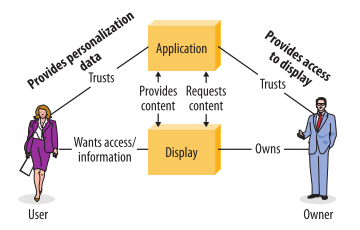
\includegraphics[width=0.7\columnwidth]{tacita.png}
\caption[Sistema \textit{Tacita}] {Sistema \textit{Tacita} ~\cite{Davies2012b}}
\label{fig:tacita}
\end{figure}

\subsection{Tipos de ligação}

Sempre que queremos interagir com determinado ecrã público e o mesmo não possuí um reconhecimento de movimento ou não é sensível ao toque, necessitamos de um dispositivo. Esse dispositivo permite-nos efetuar a ligação, esta pode ser realizada de variadas formas, seja através de SMS, QR code, Bluetooth, email, inserção de código ou acedendo a determinado link.

A interação através do toque transmite ao utilizador uma maior espontaneidade para este interagir com o respetivo ecrã, no entanto por norma é também sinónimo de piores condições de limpeza~\cite{Ballagas}.

Uma conexão usando Bluetooth também pode ser intuitiva, contudo por vezes requer que o utilizador instale software específico no seu dispositivo e o computador do ecrã público necessita de uma configuração Bluetooth de modo a aceitar a ligação~\cite{Ballagas}.

As ligações através de QR code, email, inserção de código ou link exigem que exista uma ligação à Internet para que o transeunte possa usufruir da aplicação. 
Gehring et al.~\cite{Gehring}, fazem referência ao protocolo \textit{TUIO}, esquema na figura ~\ref{fig:TUIO}, para enviar a informação do dispositivo para o ecrã. Inicialmente o ecrã precisa de ser detetado e identificado, depois o dispositivo deteta automaticamente o ecrã em direto, se os dois estiverem conectados na mesma rede. Após isto, o reconhecimento do QR code existente no local permite a emparelhar os dois dispositivos.

\begin{figure}[h]
\centering
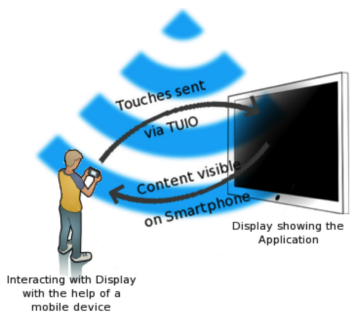
\includegraphics[width=0.7\columnwidth]{TUIO.png}
\caption[textit{TUIO} Protocolo] {\textit{TUIO} Protocolo ~\cite{Gehring}}
\label{fig:TUIO}
\end{figure}


O uso de um dispositivo clarifica o paradigma da interação, contudo providenciar dispositivos em locais públicos levanta alguma problemas relacionados com a segurança física, condições sanitárias, manutenção e o uso simultâneo, o uso do seu próprio dispositivo resolve estes problemas~\cite{Ballagas}.

\subsection{Exemplo de Arquitetura}

Como poderia uma aplicação, integrar a rede de um ecrã público? Clinch et al.~\cite{Clinch2012}  apresentam uma arquitetura composta por 4 componentes(figura~\ref{fig:arquitetura}), sendo eles:
\begin{enumerate}
\item \textbf{aplicações móveis} - permitem que os transeuntes definam as preferências da aplicação e determina a respetiva proximidade para com o ecrã;
\item \textbf{ecrãs} - para renderizar o seu conteúdo;
\item \textbf{conjunto de aplicações web} - especificamente desenvolvidas para ecrãs públicos;
\item \textbf{diretório} - para fornecer informações sobre a localização geográfica de um ecrã, 
capacidades e aplicações disponíveis.
\end{enumerate}

\begin{figure}[h]
\centering
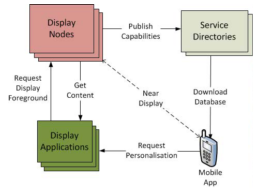
\includegraphics[width=0.7\columnwidth]{arqui.png}
\caption[Componentes da Arquitetura] {Componentes da Arquitetura~\cite{Gehring}}
\label{fig:arquitetura}
\end{figure}


\section{Aplicações para multi-utilizadores}

As primeiras aplicações desenvolvidas para múltiplos utilizadores usavam hardware caro e desenvolvido para um propósito específico, pois eram necessários dispositivos específicos que permitissem a interação com determinado computador. Atualmente essa interação torna-se mais fácil, sendo possível através de um tablet ou smartphone.
Stewart et al.~\cite{stewart1997single} lançou o termo \textit{Single Display Groupware} com a aplicação KidPad, desenvolvida para crianças, permitindo-lhes desenharem ao mesmo tempo no mesmo computador.

PebblesDraw ~\cite{Myers1998a}, desenvolvido posteriormente,  é um programa de desenho partilhado que permite a todos os seus utilizadores desenharem ao mesmo tempo, e tendo em conta que é um Single Display Groupware (SDG), estes partilham também o mesmo ecrã e consequentemente os mesmo \textit{widgets}. Esta aplicação data de 1998, ano em que o uso dos smartphones era diminuto ou mesmo inexistente, usando para a interação PDA’s, pois eram fáceis de programar, populares, e conectavam-se facilmente a um computador, independentemente do sistema operativo. 
A maneira convencional de identificar os diversos utilizadores passa por atribuir a cada um, uma cor diferente, no entanto para esta aplicação foram desenvolvidas novas técnicas de interação para suportarem de forma mais eficiente o uso simultâneo, atribuindo a cada um deles uma forma. Tal como num jogo de tabuleiro, que cada jogador escolhe o seu peão, também aqui podem escolher qual o objeto que os representa, como um quadrado, triângulo entre outros.

De modo a permitir o uso de vários utilizadores ao mesmo tempo, uma conexão através de GPRS, WiFi ou Bluetooth, será a melhor escolha em termos tecnológicos~\cite{Ballagas}.

\section{Trabalhos relacionados}
\begin{itemize}
\item \textbf{Poppet}~\cite{Vajk2008b} - é uma \textit{framework} que utiliza os sensores do telemóvel, como câmaras, acelarometros, NFC, que podem ser ligados aos jogos, para correrem nos ecrãs públicos. Foi desenvolvido para um telemóvel em específico, Nokia 5500, contudo é suficientemente genérico para funcionar corretamente com uma larga gama de telemóveis usando o bluetooth como meio de ligação. O reconhecimento dos gestos exige um estudo cuidado, pois a variação de como o utilizador manipula o dispositivo pode produzir anomalias nos outputs e não existia método de obter a posição física do mesmo no espaço real, como por exemplo acontece no comando da consola \textit{Wii}(figura~\ref{fig:poppet}).

\begin{figure}[h]
\centering
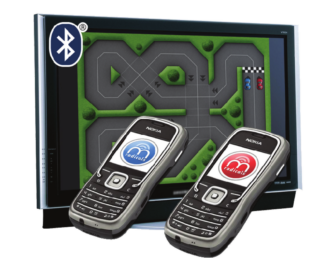
\includegraphics[width=0.6\columnwidth]{poppet.png}
\caption[Sistema \textit{Poppet}] {Sistema \textit{Poppet}~\cite{Vajk2008b}}
\label{fig:poppet}
\end{figure}

\item \textbf{PUREWIDGETS SYSTEM~\cite{Cardoso2012g}} - é composto por uma biblioteca de \textit{widgets} e \textit{web service} que permite lidar com eventos interativos. Representa um \textit{toolkit} que suporta múltiplos mecanismos de interação, eventos assíncronos e interação concorrente. Fornece abstrações de alto nível que se adequam ao tipo de interação que normalmente faz com aplicações públicas e permite que programadores se concentrem sobre o trabalho criativo de design de aplicações interessantes e experiências do utilizador. \textit{PureWidgets} suporta diferentes tipos de ligação, como SMS, email, Bluetooth naming, Bluetooth OBEX and QR codes. Para a sua implementação foi usada a plataforma \textit{Google’s App Engine} e \textit{Google’s Web Toolkit}.


\item \textbf{Super Sync Sports}\footnote{http://www.chrome.com/supersyncsports/\#/en-GB/m/tfejb} -  uma aplicação web, desenvolvida pela Google que permite ao utilizador jogar se este estabelecer uma ligação ao computador através do seu dispositivo móvel. O objetivo será assumir o papel de um desportista e terminar as diversas provas. São usadas \textit{websockets} para permitir a colaboração em tempo real, no seu desenvolvimento foi também usado HTML e CSS(figura~\ref{fig:chrome}).

\begin{figure}[h]
\centering
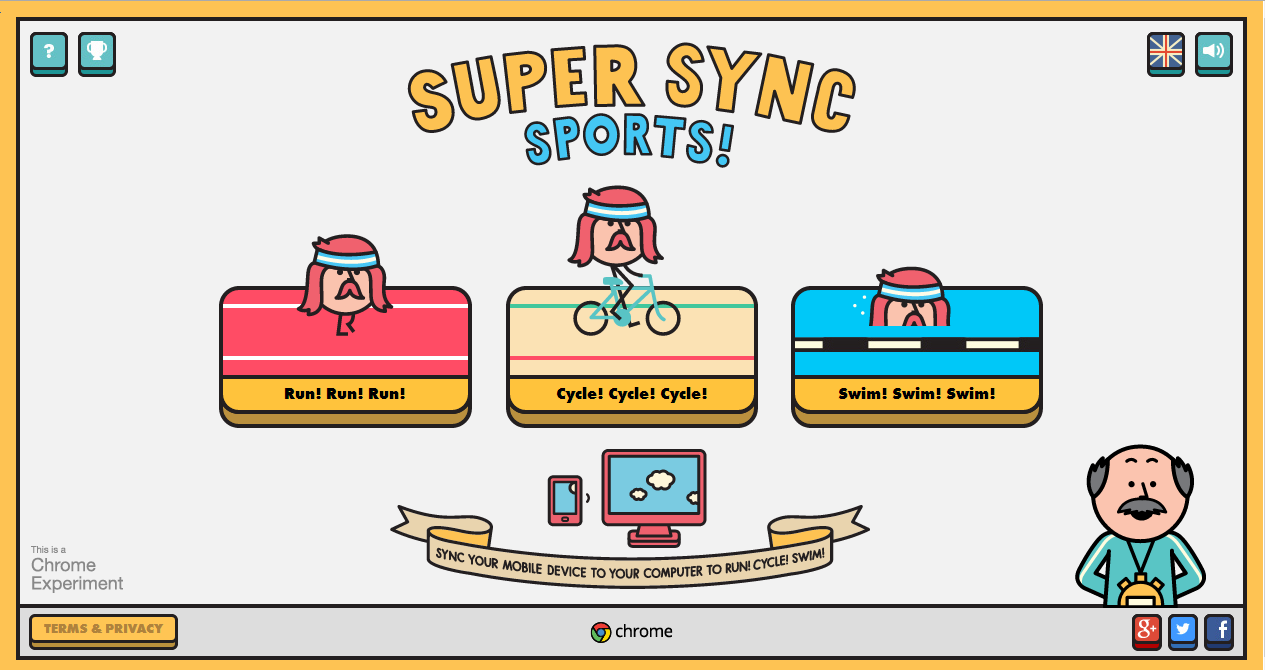
\includegraphics[width=0.6\columnwidth]{chrome.png}
\caption {Super Sync Sports}
\label{fig:chrome}
\end{figure}

\item \textbf{Stripenight Racer}\footnote{http://www.stripenight.com/racer/} - é também um pequeno jogo, que simula uma corrida de automóveis e o utilizador tem a autonomia de controlar o veiculo com o movimento do seu dispositivo, usa a mesma tecnologia para a ligação que a aplicação anterior(figura ~\ref{fig:racer}).

\begin{figure}[h]
\centering
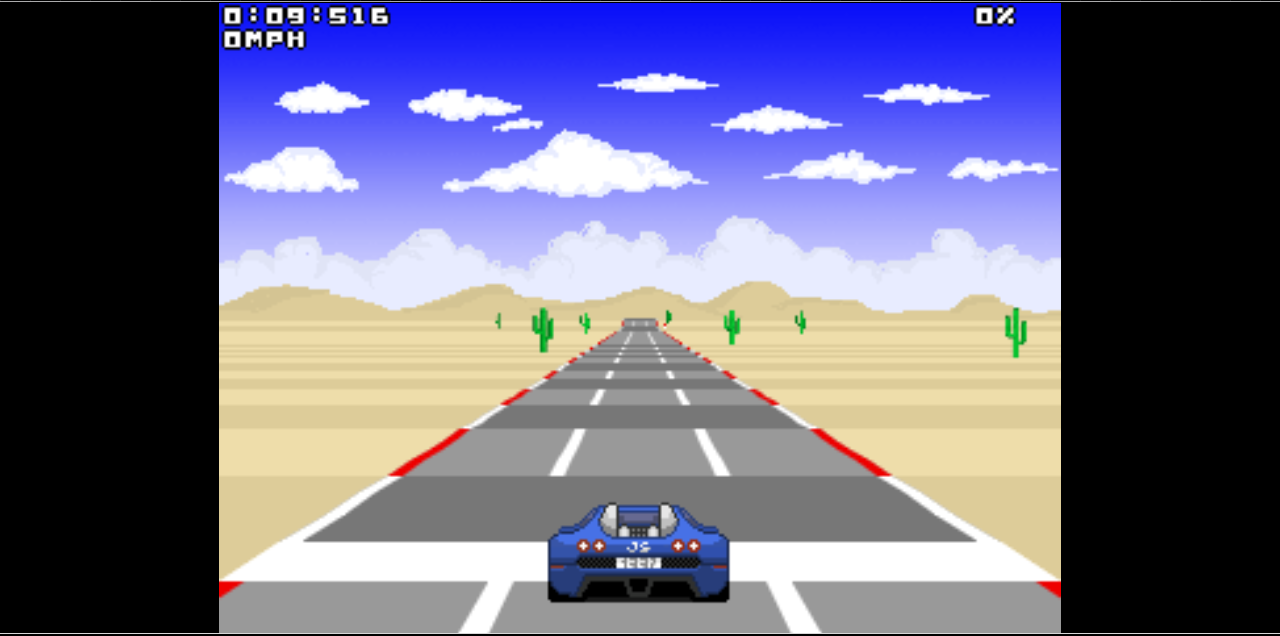
\includegraphics[width=0.6\columnwidth]{race.png}
\caption {Stripenight Racer}
\label{fig:racer}
\end{figure}

Os dois jogos apresentados, foram escolhidos pois demonstram um interação baseada no paradigma \textit{direct-manipulation}, uma vez que o utilizador vê em tempo-real as alterações conforme movimenta o seu dispositivo.


\end{itemize}

\section{Conclusões}

A realização deste capítulo permitiu a realização de uma pesquisa relacionado com o tema a desenvolver, facilitando o conhecimento e relação com os termos específicos mais usados na área.
A criação de aplicações públicas não se centra apenas no desenvolvimento das aplicações enquanto programas de computador, existe todo um conjunto de fatores a ter em conta quando se pensa numa solução possível de ser implementada.
Se a aplicação desenvolvida necessitar de um dispositivo para a interação ser possível, existem diversas formas de a conexão ocorrer, podendo ser através de SMS, QR codes, Bluetooth, email, link, etc.
É ainda possível, que as mesmas, possam ser utilizadas por várias pessoas ao mesmo tempo, o que requer cuidados específicos, quanto ao propósito da aplicação, diferenciação dos utilizadores e facilidade de adição dos mesmos.
Nenhum dos trabalhos referidos, não são o que se pretende com esta dissertação enquanto produto final, no entanto podem vir a ser uma ajuda ao longo do desenvolvimento.


	

%!TEX root = mieic.tex
\chapter{Metodologia} \label{chap:metod}

\section*{}

Neste capítulo é descrita de uma forma sucinta a metodologia que será usada para alcançar os objetivos finais, que será baseada na interação pessoa-ecrã público. É incluída uma pequena descrição, definições e terminologias e ainda as diferentes fases para atingir o desejado. 

\section{Definições e Terminologia}

Considerando o cerne da questão, será adequado considerar dois coneitos relacionados, sendo eles Interação Pessoa-Computador e Desenvolvimento Centrado no Utilizador.

IHP tenta perceber como os utilizadores interagem com um computador, foca-se em perceber qual a melhor forma de projetar os sistemas interativos de forma mais agradável para quem usufrui dos mesmos.

Existem algumas rasões que fazem com que IHP seja uma área de estudo com valor~\cite{smith2006human}:
\begin{itemize}
	\item Considera como principal no desenvolvimento de aplicações o utilizador final e preocupa-se com ele aquando da fase de desenvolvimento.
	\item Fornece uma base sobre a qual é possível avaliar métodos de design para a sua eficiência e eficácia. O desenvolvimento de um sistema necessita de várias formas de avaliar os métodos usados, que podem ser obtidos através de IHP.
	\item Proporciona um ambiente baseado no mundo real, permitindo novas teorias baseadas na psicologia humana. este campo é uma das áreas de crescimento mais rápido considerando a ciência da computação.
\end{itemize}

DCU é um conceito para descrever os projectos nos quais o utilizador final influencia a forma como um projeto se desenvolve. É ao mesmo tempo uma filosofia ampla com vários métodos, pois há diversas maneiras através das quais os utilizadores são envolvidos. Uma metodologia baseada em UCD interessa-se pelas necessidades dos mesmos e frequentemente envolve-os durante o processo de design, normalmente durante o levantamento de requisitos e testes de usabilidade~\cite{Abras2004}.


\section{Fases de Desenvolvimento}

Uma vez que a metodologia é baseada no utilizador final é importante desenvolver um sistema intuitivo e de fácil utilização aos seus utilizadores.Um desnvolvimento centrado no utilizador final pressupõe 4 fases(figura ~\ref{fig:user-center}), sendo elas:
\begin{itemize}
\item Analisar - Engloba a recolha de requisitos, tendo em conta o contexto de uso e o propósito de desenvolvimento
\item Design - Projeta possíveis soluções que cumpram o que foi definido na fase anterior;
\item Implementar - Desenvolvimento de protótipos que tornem perceptiveis as soluções idealizadas, nos quais os conceitos têm de ser implementados.
\item Validar - Avaliação, por parte de especialistas, da usabilidade e possíveis riscos tendo em conta os requisitos do utilizador final e os conceitos envolvidos.
\end{itemize} 

\begin{figure}[h]
\centering
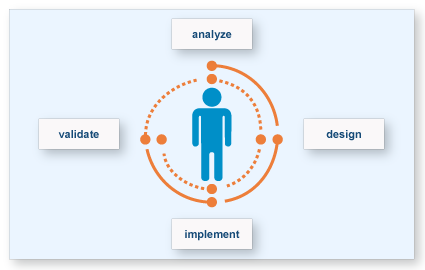
\includegraphics[width=0.7\columnwidth]{user.png}
\caption[Desenvolvimento Centrado no Utilizador] {Desenvolvimento Centrado no Utilizador\protect\footnotemark}
\label{fig:user-center}
\end{figure}

\footnotetext{http://www.medical-safety-design.de/en/medical-safety-design/user-centered-interface-design/}




 
%!TEX root = mieic.tex
\chapter{Solução Implementada} \label{chap:sol}

\section*{}

Neste capítulo é descrita de forma pormenorizada a solução implementada de modo a responder aos desafios colocados na introdução, cumprindo assim os objetivos propostos.
Inicialmente é caracterizada a arquitetura definida, fazendo referência aos diferentes modulos que constituem o “produto” final. Posteriormente são referidas de uma forma breve as tecnologias envolvidas no seu desenvolvimento.


\section{Visão Geral} \label{sec:geral}

Tal como foi referido na definição dos objetivos, era esperado o desenvolvimento e validação de uma arquitectura que permitisse uma interação baseada na manipulação direta, através de um dispositivo móvel, facilitando a criação de aplicações para ecrãs públicos.  
Na solução encontrada, de uma maneira global, é possível diferenciar três diferentes componentes, sendo eles o servidor, desenvolvido em node.js, a aplicação, que irá correr no servidor criado comunicando com este através de \textit{web sockets} e ainda o utilizador final, aqui identificado como cliente.
A FIGURA apresenta, de uma forma simples, os componentes acima descritos.
\missingfigure{Diagrama de componentes}

A [inserir num fig] representa um diagrama de sequência mostrando as diferentes interações entre os componentes constituintes do sistema implementado. Inicialmente terá de existir um pedido por parte de um ecrã para aceder à aplicação, neste momento a aplicação comunica com o servidor e a partir daqui está preparada para pedidos de possíveis utilizadores. Um utilizador, ao querer interagir com a aplicação está a enviar um pedido para esta, que por sua vez avisa o servidor e este é responsável por mostrar no dispositivo o widget da aplicação. Neste momento o widget liga-se ao servidor e após ocorrer a ligação procede-se à troca de “mensagens” que permitem ao utilizador definir o seu nome, quando o cliente tiver o nome definido pode usufruir do widgets disponíveis, realizando-se a comunicação do  widget para o servidor, que por sua vez envia para a aplicação.
\missingfigure{Diagrama de sequência}


\section{Tecnologias Usadas} \label{sec:tec}

Ao longo da implementação houve necessidade de optar por diversas tecnologias para que fosse possível alcançar o objetivo desejado, Node.js foi usado para a implementação do servidor e \textit{web sockets} e \textit{socket.io} para facilitar a comunicação entre os diversos componentes. Foi também usada a \textit{framework} \textit{Prototype} que pemrite a manipulação de classes em \textit{JavaScript}, e uma biblioteca, \textit{Swipeable} que dá resposta a eventos swipe facilitando a utilização.

\begin{itemize}

\item \textbf{Node.js}


\textit{Node.js} é uma plataforma construída para facilitar o desenvolvimento de aplicações de alta escalabilidade em tempo real, com base no interpretador \textit{Javascript V8} da \textit{Google}, que antes da execução compila \textit{JavaScript} em código máquina, melhorando consideravelmente o tempo de execução. Deste modo Node permite a construção de aplicações rápidas e altamente concorrentes.

Segundo Michael Abernethy ~\cite{Abernethy2011} node altera a noção de como um servidor deve funcionar, referindo que o seu objetivo é permitir que um programador construa applicações com grande escalabilidade e que o código desenvolvido suporte milhares de ligaçõe simultâneasa numa só máquina. 

\textit{Node.js} opera uma \textit{thread} simples, usando chamadas E/S “que não bloqueiam”(non-blocking), permitindo o suporte das diversas ligações ~\ref{fig:node}.

\begin{figure}[ht]
\centering
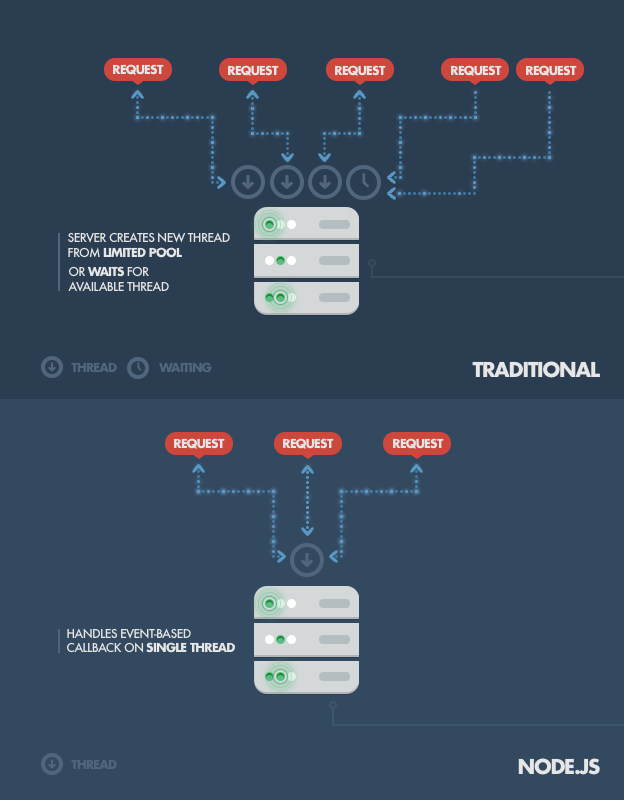
\includegraphics[width=0.5\columnwidth]{node.png}
\caption[\textit{Node.js}] {Diferença entre técnicas tradicionais de servidores e \textit{Node.js}\protect\footnotemark}
\label{fig:node}
\end{figure}

\footnotetext{http://www.toptal.com/nodejs/why-the-hell-would-i-use-node-js}

\item \textbf{Web Sockets}

De forma a permitir a comunicação do utilizador, lado do cliente, com o servidor criado foram usados web sockets. Estes foram desenvolvidos para serem implementados em em aplicações ou servidores web, usando um protocolo independente baseado em TCP.

O protocolo websocket encontra-se standardizado, o que significa que é seguida uma norma no envio de informação entre o servidor e o “browser” sem que haja uma solicitação por parte do cliente o que possibilita uma maior interação entre estes, facilitando a criação de aplicações em tempo real. É deste modo criada uma ligação bi-direcional entre o \textit{browser} e o servidor, pois a conexão é mantida aberta enquanto as mensagens são encaminhadas de um lado para o outro.


\item \textbf{Socket.io}

Socket.io é descrita como uma biblioteca javascript usada no desenvolvimento de aplicações web. Esta é composta por 2 partes, uma biblioteca para o lado do cliente, que corre no browser, e outra para o lado do servidor, que para terá de ser implementado em node.js, daí este estar acima referido como uma das tecnologias usadas. Quer o lado do cliente quer o do servidor apresentam “API’s” idênticas. 
Usa, principalmente como protocolo, websockets, também escolhido como tecnologia usada no desenvolvimento desta solução, contudo, se necessário, podem ser utilizados outros, como por exemplo Adobe Flash sockets, JSONP polling, and AJAX long polling. 
A sua escolha aliada a websockets fornece bastante recursos, como a transmissão para múltiplos sockets, armazenamento de informação associada a cada cliente e ainda “inputs/outputs” assíncronos. 

\item \textbf{Prototype}

Prototype é uma \textit{framework} em \textit{JavaScript} que fornece algumas funções para o desenvolvimento de aplicações em \textit{JavaScript}. As suas funcionalidades variam entre pequenos atalhos de programação e principais funções para lidar com \textit{XMLHttpRequest}.

Esta \textit{framework} fornece ainda uma biblioteca com funções que suporta classes e objetos baseados em classes, algo que não é possível em \textit{JavaScript}.

\item \textbf{Swipeable}

Swipeable trata-se de uma biblioteca que permite obter resposta a eventos \textit{swipe} realizados num dispositivo \textit{touch}, sendo uma abstração do \textit{touchstart}, \textit{touchmove} e \textit{touchend}. 
Foi incluída no ficheiro widget.js de para possibilitar o desenvolvimento e correto funcionamento do widget “SWIPE”.

\end{itemize}


\section{Framework Desenvolvida} \label{sec:framework}

\subsection{API}

\subsection{Controlos Definidos}

	A API desenvolvida apresenta três diferentes tipos de controlos que o programador terá à sua disposição para implementar, de acordo com aplicação desenvolvida. Neste momento existem como possíveis opções, o \textit{joystick}, o \textit{swipe} e ainda outro composto por uma caixa de introdução de texto.

	\begin{itemize}

	\item \textbf{Joystick}

		Controlo composto pelas quatro setas tradicionais, esquerda, direita, cima e baixo, que pode ser utilizado em qualquer aplicação que exija uma movimentação.

	\item \textbf{Swipe}

		Controlo que usa as propriedade touch do dispositivo para controlar a aplicação, definido apenas para reconhcer uma direção, contudo pode ser alterado.

	\item \textbf{InputText}

		Controlo que permite ao utilizador a interação com aplicações que exijam a introdução de texto.

	\end{itemize}


	
\subsection{Aplicações Exemplo}

	Neste momento apenas existe uma aplicação exemplo, no entanto permite ao utilizador o uso dos três tipos de controlo disponíveis.
	



 
%!TEX root = mieic.tex
\chapter{Testes} \label{chap:testes}

\section*{}

A realização de testes é uma fase importante no desenvolvimento de qualquer produto, permitindo descobrir alguma falhas no trabalho efetuado e dando sugestões de melhorias futuras.
Neste capítulo são descritos os diversos tipos de testes executados, bem como as conclusões a que os mesmos permitiram chegar.

\section{Testes Iterativos}

	Ao longo de todo o desenvolvimento, sempre que uma nova funcionalidade era implementada surgia a necessidade de a testar, de forma a perceber se esta efetuava a ação desejada.

	Este tipo de testes, permite a quem está a desenvolver a aplicação, obter de forma rápida \textit{feedback} do trabalho acabado de realizar, prevenindo erros futuros semelhantes e trabalho desnecessário.

	Por exemplo, na solução implementada, aquando da criação dos tipos de controlo, primeiro foi definido e implementado apenas um, neste caso a \textit{widget joystick}, que foi testado verificando se a comunicação com a aplicação existia, e se as setas executavam no jogo as ações supostas. Assim, qualquer erro detetado e corrigido contribuiu para uma maior facilidade na criação das restantes \textit{widgets}, diminuindo a correção de erros no final da implementação.


\section{Testes Finais}
	
	Os testes para verificar se as funcionalidades implementadas correspondiam ao especificado inicialmente são de fácil realização e apenas requerem que alguém experimente o que foi desenvolvido. Contudo neste projeto era também importante perceber de que modo outros programadores poderiam usar a \textit{framework} desenvolvida com o intuito de definirem alguns tipos de controlo para as sua próprias aplicações.

	Para a realização destes testes foram escolhidos três estudantes do 5º ano do Mestrado Integrado em Engenharia Informática e Computação. Ao longo do seu percurso académico tiveram duas unidades curriculares onde fizeram \textit{web development} e tiveram de interagir com \textit{HTML5}, \textit{CSS3} e \textit{JavaScript}.

	Um dos elementos, o sujeito A, apenas possuía a experiência adquirida durante o percurso académico. Os outros dois elementos,  os sujeitos B e C, já tinham realizado alguns projetos extra-curriculares que os obrigou a explorar um pouco mais estas tecnologias, fornecendo-lhes uma maior experiência e conhecimento. 

	Inicialmente, foram explicados aos intervenientes os objetivos do projeto, para que eles estivessem enquadrados e pudessem perceber o seu papel nesta atividade. Também lhes foi dada, antes de iniciarem, uma breve explicação sobre o que teriam de fazer para usar a \textit{framework}.

	De seguida, foi-lhes dado todo o projeto desenvolvido, com a exceção de dois ficheiros. Um que continha o código do jogo implementado e o outro que dizia respeito à implementação dos controlos pretendidos.

	O objetivo era que desenvolvessem uma pequena aplicação e que usassem para a definição dos controlos exigidos a \textit{API} desenvolvida. Os participantes dispunham de 2 horas e 30 minutos para a realização desta atividade. O tempo dado foi utilizado de maneiras diferentes pelos participantes. Enquanto o utilizador A apenas se preocupou em implementar uma solução, os outros dois tiveram a preocupação de fazer perguntas pertinentes sobre a \textit{framework} e sugerir alterações.

	Das pessoas acima referidas, todas optaram pela implementação de jogos, contudo escolheram exemplos diferentes. Na tabela ~\ref{table:Resultados}, é possível ver as aplicações escolhidas, bem como um pequeno resumo das soluções obtidas.

	\begin{table}[ht]
	\centering
	\caption{Resultados Obtidos}
	\begin{tabular}{ l l l l }
	\hline
	\textbf{Elemento} & \textbf{Aplicação} & \textbf{Funcional} & \textbf{Multi-Utilizador} \\ 
	\hline
	\textbf{A} & Jogo da Forca & Sim & Não \\
	\hline
	\textbf{B} & Corrida de automóveis & Sim & Sim \\
	\hline
	\textbf{C} & Tetris & Sim & Não \\
	\hline
	\end{tabular}

	
	\label{table:Resultados}
	\end{table}

	Em todos os exemplos, os estudantes conseguiram com sucesso implementar os tipos de controlo existentes e ter uma aplicação funcional contudo, em todos eles foram referidas pequenas falhas ou sugestões relativas ao projeto.

	O decorrer dos testes permitiu obter diferentes opiniões de acordo com o desenvolver da solução:

		\begin{itemize}
		\item \textbf{Jogo da forca: } Só foi usado o controlo que exigia introdução de texto. O utilizador inseria o seu nome de jogador e poderia começar a jogar.

		Só foi conseguida a versão para um jogador.

		\item \textbf{Corrida de automóveis: } Foi implementada com sucesso, sendo possível usar os três diferentes tipos de controlo, começando por introduzir o nome de jogador, seguido da escolha da \textit{widget} preferido para controlar o veículo.

		A solução apresentada suportava o modo multi-jogador, em que os jogadores eram distinguidos pela cor do automóvel e respetivo nome.

		Foi sugerida a criação de um novo tipo de controlo que usasse o acelerómetro do dispositivo, de modo a permitir uma interação através do movimento do mesmo.

		\item \textbf{Tetris: } À semelhança dos anteriores, também este exemplo se encontrava funcional no fim do tempo dado. Foram usados dois diferentes tipos de controlo, a caixa de texto para a escolha do nome do utilizador e o \textit{joystick} para controlar as peças do jogo. 

		Tal como aconteceu no exemplo do jogo da forca, este apenas podia ser jogado por um utilizador. A pessoa que o implementou possuía a solução para permitir um modo multi-jogador, no entanto, por falta de tempo não houve a possibilidade de implementar. A solução passaria pela existência de um número de ``tabuleiros'' de tetris igual ao número de jogadores.

		\end{itemize}

	Adicionalmente, foram também sugeridas pequenas alterações a nível de funções da \textit{API} desenvolvida que foram corrigidas. O método \textit{setOptions(options)}, que permite ao programador alterar a informação que é enviada através da \textit{widget}, inicialmente estava definido para cada \textit{widget} independentemente. Após a realização dos testes, foi sugerido pelo sujeito B, que faria sentido ser um método geral, uma vez que a informação enviada, independentemente do tipo de controlo seriam iguais para determinada aplicação.
	O sujeito C sugeriu que seria preferível o programador não ter de seguir um estrutura específica para o ficheiro \textit{HTML}, pois condiciona a liberdade do mesmo. 

	Ainda durante a realização destes testes foi possível constatar que existem algumas alterações a efetuar no código original para a implementação de novas aplicações, o que dificulta o trabalho de futuras pessoas que não estejam familiarizadas com código fornecido. Por exemplo, é necessário alterar três vezes o endereço onde a aplicação está a correr, o que deveria ser evitado para que futuros utilizadores não necessitem de alterar ficheiros exteriores à \textit{framework}. É também necessário que o programador preste especial atenção ao ficheiro \textit{index.js}, local onde são chamadas funções específicas da aplicação implementada. 

\section{Testes Públicos}

	Aquando da definição e especificação do projeto foi referido que seria vantajoso testar a solução implementada em ecrãs públicos, no entanto, devido a algum atraso no desenvolvimento, o mesmo não foi possível.

	A realização destes testes permitiria tirar algumas conclusões relativas à utilização por parte dos transeuntes, que poderiam ser resposta às seguintes questões:

	\begin{itemize}
	\item \textbf{Antes de efetuar a ligação com o ecrã:}
		\begin{itemize}
		\item Que riscos estou a correr se me ligar a este ecrã?
		\item O que tenho de fazer para me conseguir ligar?
		\end{itemize}
	\item \textbf{Após estar conectado com o ecrã}:
		\begin{itemize}
		\item O que tenho de fazer para usar a aplicação?
		\item Como sei quem sou eu durante a interação?
		\item O que faço quando desejar terminar?
		\end{itemize}
	\end{itemize} 

\section{Conclusões}

	Após a realização dos testes previamente descritos, houve a possibilidade de perceber realmente de que modo a aplicação era vista por alguém que não estava a par do seu desenvolvimento e que alterações deveriam ser efetuadas para obter uma melhor \textit{performance}.

	A sua realização permitiu descobrir falhas que puderam ser corrigidas ainda antes de se dar por concluída a solução final e outras que ficaram registadas como melhorias a efetuar caso exista a hipótese de dar continuidade ao trabalho realizado.

	A realização dos últimos testes referidos poderá acontecer em qualquer altura sendo apenas necessário a existência de infra-estruturas adequadas.



	

 
%!TEX root = mieic.tex
\chapter{Discussão Crítica} \label{chap:disc}

\section*{}

Ao longo de todo o processo de desenvolvimento, para além do cumprimento dos objetivos foi também importante perceber de que modo seria possível alcançá-los de forma eficaz e que tecnologias deveriam ser usadas.

O desenvolvimento de aplicações de cariz público levanta algumas questões, que no momento do desenvolvimento têm alguma importância nas escolhas efetuadas.

\subsection*{Escolhas tecnológicas}

Quando se fala de tecnologia é de conhecimento geral que a maior parte das vezes, para a mesma finalidade existem diversas opções, deste modo é necessário ponderar e perceber qual delas se enquadra melhor na solução pretendida e se os resultados finais que serão obtidos correspondem ao que é desejado.

Uma vez que o projeto exigia que existisse uma comunicação entre o dispositivo do utilizador final e a aplicação, que o mesmo controlaria, e que no momento da interação, poderia existir mais do que um cliente, levou ao uso da biblioteca \textit{Socket.io}, em conjunto com o protocolo \textit{websocket}. Estes criam uma ligação bi-direcional, mantendo a conexão aberta enquanto as mensagens são encaminhadas de um lado para o outro, permitindo a transmissão de informação para múltiplos \textit{sockets}, o armazenamento de informação associada a cada cliente e ainda \textit{inputs/outputs} assíncronos. 

Posteriormente, no desenvolvimento da API que daria origem aos \textit{widgtes}, era pretendido o uso de classes e também herança, de modo a que todos os tipos de controlo tivessem uma construção semelhante e que a sua implementação se tornasse mais intuitiva para futuras aplicações, no entanto \textit{JavaScript} não suporta a manipulação de classes nem objetos baseados nas mesmas. Esta característica de \textit{JavaScript} leva à introdução da \textit{framework} \textit{Prototype.js} na solução.

Outra questão que exigiu uma reflexão mais cuidada e consequente tomada de decisão centrou-se no que o transeunte teria de fazer para que se conseguisse ligar a um ecrã e usufruir da aplicação. A escolha recaiu sobre a leitura de um \textit{QR code}. 

Apesar desta decisão ter como desvantagem a obrigatoriedade de o utilizador possuir no seu dispositivo um leitor de \textit{QR codes}, por outro lado é algo que desperta o interesse de quem passa por um ecrã, que quando se apercebe da sua existência a sua curiosidade leva-o a querer experimentar. Segundo Wilson~\cite{Wilson2014}, estes são referidos como algo bastante simples de usar, que recorre a poucos recursos, como tempo e dinheiro, e mesmo com uma fraca aceitação por parte do público em geral, trata-se de uma tecnologia demasiado simples para ignorar.

O uso das restantes tecnologias surge quase implicitamente ao longo do desenvolvimento, conforme os objetivos que se pretendiam alcançar.

\subsection*{Exemplo Implementado}

Era pretendido encontrar uma solução para os desafios relacionados com o tema proposto que são descritos na introdução. Foi solucionada a questão relacionada com a utilização da aplicação por um ou mais utilizadores, bem como os diferentes tipos de controlo que serão suportados.

O desenvolvimento da aplicação para a prova do conceito não fazia parte do contexto da dissertação, podendo integrar-se um exemplo já existente com a API desenvolvida. Consequentemente, a escolha efetuada surge com base numa pesquisa de jogos desenvolvidos em \textit{JavaScript}, que permitissem o modo multi-jogador. 

Optou-se pelo clássico jogo da \textit{Snake}, por ser um jogo conhecido, que não necessita de instruções extensas, permite uma interação rápida, sendo desafiante e no caso de multi-jogador torna-se competitivo. O exemplo encontrado só continha o modo de jogo individual, no entanto foi fácil a sua alteração para que houvesse a possibilidade de mais do que uma pessoa jogarem ao mesmo tempo.

No exemplo implementado, tal como já foi referido, os diferentes utilizadores são distinguidos com base na cor da cobra que os representa durante o jogo e ainda conseguem identificar-se inserindo logo no início o seu nome de utilizador. 

Esta é apenas uma das possibilidades encontradas para dar resposta à distinção num sistema que suporta multi-utilizadores. No entanto, outras hipóteses poderiam ser usadas, estando esta característica bastante dependente do tipo de aplicação a implementar. No caso de se tratar de um sistema colaborativo, a distinção é mais fácil se for atribuída aos jogadores uma maneira de eles próprios escolherem a sua identificação, seja através de uma cor, de um nome ou até um objeto que os identifique. Se, por outro lado, for um sistema independente onde cada utilizador necessita do seu espaço será mais vantajosa a divisão do ecrã em partes iguais para cada um.

Na solução apresentada estão disponíveis três diferentes tipos de controlo, que, tal como já foi referido representam um \textit{joystick}, uma caixa para introdução de texto e ainda \textit{swipe}. A seleção destes ocorreu na tentativa de abranger um grande número de aplicações, não sendo necessária a criação de novos \textit{widgets} para que um programador consiga criar aplicações interativas. 

Inicialmente foram apenas definidos o \textit{joystick} e o \textit{widget}, o \textit{swipe} apesar de ter a mesma funcionalidade que o \textit{joystick} surge de forma a fornecer outra alternativa ao utilizador recorrendo aos recursos disponíveis no seu dispositivo. 
Julie Rico em ~\cite{Rico2010}, conclui que uma experiência positiva aumenta a recetividade a controlos gestuais, neste caso concreto os movimentos de \textit{swipe}, levando à repetição.  


\subsection*{Testes Realizados}

Os testes realizados já quase no fim do desenvolvimento foram uma etapa importante que permitiram fazer um balanço do que tinha sido implementado.

Através destes foi possível entender que apesar dos controlos definidos serem bastante abrangentes existem outras possibilidades que seriam uma mais valia na \textit{framework} desenvolvida, dando resposta a um maior número de aplicações. Uma vez que os testes apenas foram efectuados quase na recta final do projeto, não houve tempo para esta melhoria, ficando assim como possível trabalho futuro.

A sua realização permitiu ter uma visão externa, sugerindo alterações que para quem esteve no desenvolvimento da solução, muito provavelmente, passariam despercebidas. Algumas destas sugestões foram consideradas e procedeu-se à alteração ainda antes da entrega final, outras ficaram registadas para que se possa proceder à sua execução.

Desta forma, pode-se concluir, que a \textit{framework} desenvolvida, pode ainda ser melhorada facilitando ainda mais o desenvolvimento de aplicações a ser utilizadas num ambiente público.









 

%%----------------------------------------
%% Final materials
%%----------------------------------------

%% Bibliography
%% Comment the next command if BibTeX file not used, 
%% Assumes that bibliography is in ``myrefs.bib''
\PrintBib{myrefs}

%% Comment next 2 commands if numbered appendices are not used
\appendix
\include{appendix1}

%% Index
%% Uncomment next command if index is required, 
%% don't forget to run ``makeindex mieic'' command
%\PrintIndex

\end{document}
